\chapter{The CMS pixel barrel detector}
\label{ch:BPix}

This chapter presents a detailed description of the CMS pixel barrel detector.
It was developed, designed and built at the Paul Scherrer Institute (PSI) in cooperation with Eidgen{\"o}ssische Technische Hochschule (ETH) Zurich and the University of Zurich (UZH).
In this chapter, the main components of the detector are introduced. In particular, Section~\ref{sec:BPix_design} provides an overview of the detector design and mechanical structure, followed by a detailed description of the detector module and its main building blocks (Section~\ref{sec:BPix_modules}). In Section~\ref{sec:BPix_DAQ}, the detector readout and control system of the detector are explained.
The last section provides an introduction to the structure and functionality of the pixel online software (POS) used for controlling and calibrating the detector.
The calibration procedure and the results obtained for the detector commissioning for Run~2 will be described in the next chapter.
%this probably goes to the introduction
%The CMS pixel detector allows for high precision tracking in the region closest to the inter- action point in a particularly harsh environment characterized by a high track multiplicity and heavy irradiation. The main purpose of the pixel detector is the reconstruction of sec- ondary vertices from heavy flavor and tau decays and the generation of track seeds for track reconstruction.
%The detector was installed in 2008 and it has been in operation for the whole first LHC run. During LS1 it was temporarily installed in the clean room of LHC-P5, where the CMS detector is located.
%The detector has been re-installed in December 2014 and commissioned for Run~2 in January 2015. It took data successfully for the whole 2015 and it will be replaced with the Phase 1 detector in March 2016.

%%%%%%%%%%%%%%%%%%%%%%%%%%%%%%
\section{Design}\label{sec:BPix_design}
%%%%%%%%%%%%%%%%%%%%%%%%%%%%%%

The CMS BPix detector~\cite{Kastli2007724} consists of three cylindrical layers at mean radii of 4.4, 7.3 and 10.2\cm from the center of the detector and with a length of 53\cm.
A three dimensional representation of the detector can be seen in Fig.~\ref{fig:PixLayout_a}.
The layers are composed of 768 modular detector units that consist of thin segmented silicon sensors, with a pixel size of $100\times150$\unit{m$^2$} providing about 48 million readout channels.
The pixels are almost square shaped in order to achieve a similar track resolution in both the $r\phi$ and $z$ direction.

\begin{figure}[!htb]
 \begin{center}
 \subfigure[]{\label{fig:PixLayout_a}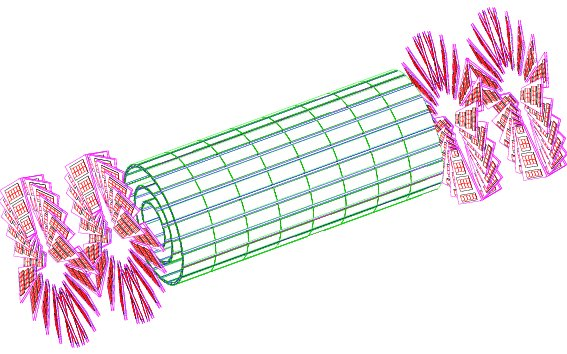
\includegraphics[width=0.6\textwidth]{\chfourteen/PixLayout.jpg}}
 \subfigure[]{\label{fig:PixLayout_b}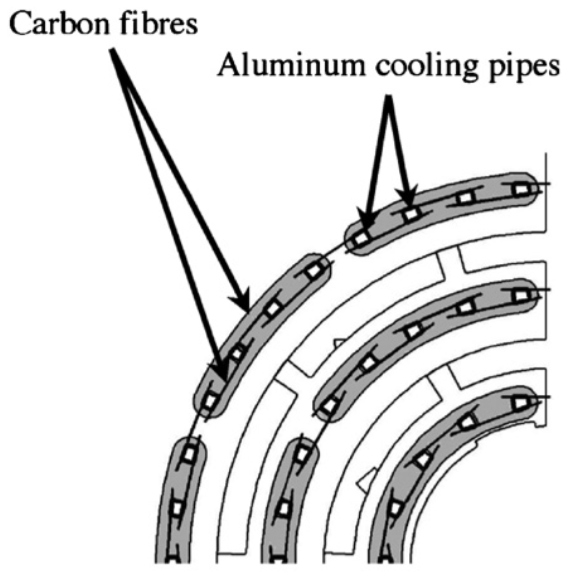
\includegraphics[width=0.35\textwidth]{\chfourteen/BPixLadders.png}}
 \end{center}
 \caption{(a) Layout of the CMS pixel detector with three barrel layers (green) and four forward disks (red). (b) Detailed view in $r\phi$ of the geometric layout.}
 \label{fig:PixLayout}
\end{figure}

Sets of 8 modules are screwed on 0.25\mm thin carbon fibre ladders that are glued to aluminium cooling pipes with 0.3\mm wall thickness.
Ladders are arranged on the layer half shells, of which three are mounted together at the end flange building up half of the BPix detector.
The total number of ladders per half shell is 10 for layer 1, 16 for layer 2 and 22 for layer 3.
To guarantee full spatial coverage ladders are mounted with overlap on alternating sides of the cooling tubes. This is shown in Fig.~\ref{fig:PixLayout_b}.
%The ladders are arranged such that the modules of two adjacent ladders overlap in order to guarantee full coverage of the interaction point (Fig.~\ref{fig:PixLayout_b}).
%Furthermore, the ladders are mounted such that the module orientation alternates between facing inward and outward in order to facilitate the mounting procedure.
The two half barrels are mechanically separated and the half shells are joined together with special ladders equipped with half modules.
The overall layout results in 96 half modules and 672 full modules.

The BPix detector is connected to four 2.2\unit{m}-long supply tube half-cylinders that carry the services along the beam pipe, accommodate the cooling lines and house the electronics for detector readout and control. The supply tubes are a complex system in design as well as in production due to the thin radial shell thickness (1--2\unit{cm}), the large number of circuits, plugs and sensors, and the fine wires and thin printed circuit boards that were used. The detector and the supply tubes are connected via a six layer PCB which is mounted on the detector end flange and distributes the power and the control signals to the individual modules.
%The final BPix system consists of four independent half cylinders depending on the position along the $z$ coordinate, $+z$ and $-z$, and on the position with respect to the center of the LHC ring, inner ($+x$) and outer ($-x$). 
The final BPix system consists of two independent half cylinders placed at $+x$ (inner) and $-x$ (outer) coordinates,
with each half shell connected to two supply tubes placed at $+z$ and $-z$ coordinates.

%but the achieved hit resolution is better because the hit reconstruction determines the barycentre of the charge that is deposited in multiple pixels. Charge sharing is ensured even when charge deposition occurs in only a single pixel by exploiting the Lorentz drift of the charge carriers in the magnetic field of CMS. The detector employs zero suppression of pixel hits using a detection threshold to reduce the required bandwidth. Additionally, data are only read out for events that are selected by the CMS trigger. This means that the detector has to buffer the data for the duration of the trigger latency.
%Multiple scattering of particles affects the momentum and impact parameter resolution of the reconstructed tracks. Because of the close proximity to the interaction point, it is fundamental that the detector contributes as little as possible to this effect. For this reason it is designed with a material budget that minimizes its effective radiation length. 
%Furthermore, the sensor and front-end electronics are designed to achieve high radiation hardness.

%%%%%%%%%%%%%%%%%%%%%%%%%%%%%%
\section{Detector modules}\label{sec:BPix_modules}
%%%%%%%%%%%%%%%%%%%%%%%%%%%%%%

The BPix modules are made of a thin, segmented silicon sensor~\cite{Allkofer200825} with a dimension of $66.6\times18.6\mm^2$ that enables the detection of particles that pass through it by measuring the ionization charge that they produce.
The charge measurement is performed by readout chips (ROCs)~\cite{Kastli:2005jj} that are connected to the sensor using the bump bonding technique with Indium solder.
Full modules consist of two rows of 8 ROCs, while half modules use a smaller sensor with $1\times8$ readout chips.
Each ROC has a size of $8\times8\mm^2$ and reads a matrix of 4160 pixel readout channels.
Table~\ref{tab:Nmodules} summarizes the configuration of full and half modules on the three different BPix detector layers.
The ROCs are wire-bonded to a three layer high density interconnect (HDI) flex printed circuit glued onto the backside of the sensor.
Mounted on the top of the HDI, a token bit manager (TBM) chip~\cite{Bartz:920426} controls the readout of the ROCs, receives all external control signals and distributes them to the chips.
Base-strips made of 250\mum thick silicon nitride (Si$_3$N$_4$) are glued underneath the ROCs allowing the module to be mounted on the mechanical support structure.
A power cable consisting of 6 copper coated aluminum wires is soldered to the HDI and brings analog, digital and high voltage to the module.
The control and readout signals are sent through a two layer Kapton signal cable which is wire-bonded to the HDI.
Additionally, the HDI distributes the signals and the voltages to the ROCs.
The modules are attached to cooling frames, with the cooling tubes being an integral part of the mechanical structure.
The size of a full module is $66.6\times26\mm^2$ and the weight is up to 3.5\unit{g} depending on the length of the signal and power cables.
The average power consumption of a full module is 2\unit{W}. An exploded view of the BPix module is shown in Fig.~\ref{fig:BpixMod}.

\begin{table}[!htb]
  \caption{\small Number of modules, readout chips and pixel channels for the three detector layers.}
  \smallskip
  \centering
  \begin{tabular}{|c|c|c|c|c|}
    \hline
    {\bfseries radius} & {\bfseries full modules} & {\bfseries half modules} & {\bfseries ROCs}  & {\bfseries pixels}  \\
    {\bfseries (cm)}   & {\bfseries \#          } & {\bfseries \#          } & {\bfseries \#  }  & {\bfseries (10$^6$)}\\ \hline \hline
    4.4                & 128                      & 32                       & 2304              & 9.6     \\
    7.3                & 224                      & 32                       & 3840              & 16.0      \\ 
    10.2               & 320                      & 32                       & 5376              & 22.4    \\
    Total              & 672                      & 96                       & 11520             & 48      \\ \hline
  \end{tabular}
  \label{tab:Nmodules}
\end{table}

\begin{figure}[!htb]
 \begin{center}
 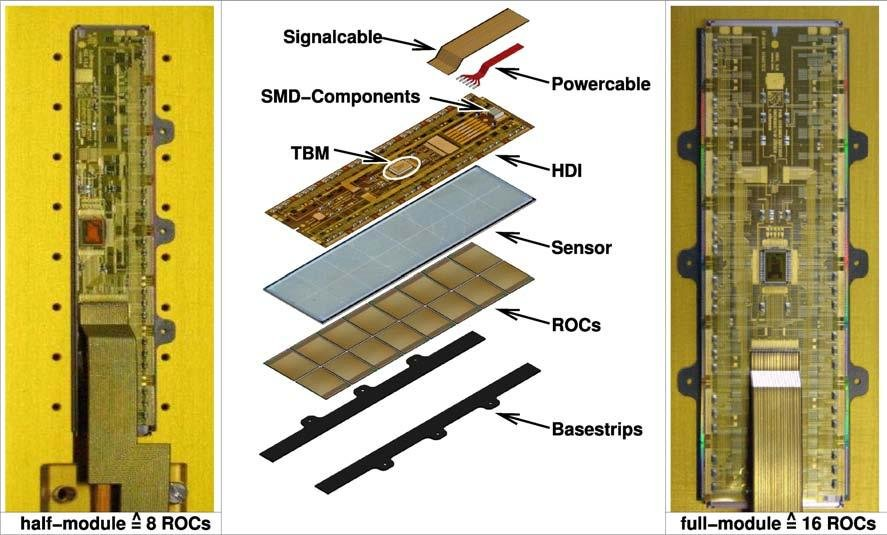
\includegraphics[width=0.6\textwidth]{\chfourteen/pixelModule.jpg}
 \end{center}
 \caption{Picture of a BPix half module (left) and full module (right). In the center, the components of a pixel barrel detector module are shown. From top to bottom: the Kapton signal cable, the power cable, the HDI, the silicon sensor, the 16 ROCs and the base strips.}
 \label{fig:BpixMod}
\end{figure}

\subsection{Sensor}

%The sensor is a planar silicon detector built with the $n^+-in-n$ technique. It is made from a $n$-type silicon wafer with a thickness of 285\mum.
The sensor is made from a $n$-type silicon wafer with a thickness of 285\mum.
Charged particles that travel through the sensor material leave electron-hole pairs as the result of multiple interactions with the atoms in the material.
For charged particles at intermediate energies ($0.1 \leq \beta\gamma \leq 1000$), the average energy loss $dE$ in a thickness $dx$ of material is described by the {\it Bethe-Bloch formula}

\begin{equation}
- \left\langle\frac{dE}{dx}\right\rangle = 4\pi N_Ar_e^2m_ec^2 z^2\frac{Z}{A}\frac{1}{\beta^2}\left[ \frac{1}{2}\ln\frac{2m_ec^2\beta^2\gamma^2W_\mathrm{max}}{I^2} - \beta^2 - \frac{\delta(\beta\gamma)}{2}\right].
\end{equation}

In the above equation, $N_A$ is the Avogadro's number, 
$r_e$ the classical electron radius,
$m_e$ the electron mass,
$z$ the charge of the particle,
$Z$ ($A$) the atomic number (mass) of the material ($Z = 14$ and $A = 28.1$\unit{u} for silicon),
$W_\mathrm{max}$ the maximum energy transfer to an electron in a single collision,
$I$ the mean excitation energy,
and $\delta$ a density effect correction.
At a particle velocity $\beta \approx 0.96$ ($\beta\gamma \approx 3$) a broad minimum is reached. At higher energies the logarithmic term leads to a slow rise again, which is eventually canceled by the density correction. A particle with an energy loss in the minimum is called a minimum ionizing particle (MIP).

The energy loss in a finite medium is subject to statistical fluctuations well described by a {\it Landau distribution} as shown in Fig.~\ref{fig:Landau}.
If a particle is not stopped in the medium, the energy loss (and therefore the number of charge carriers) varies around the peak of the distribution.
In rare but measurable cases ($\delta$-rays or $\delta$-electrons), the transferred energy is large, so that these cases are responsible for the asymmetric long tail towards high charge deposits.
Due to this tail the most probable value of energy transfer is about 30\% lower than the average value.
For a MIP crossing the sensor at an angle of $90^\circ$ the most probable number of electron-hole pairs generated in 1\mum of silicon is 76.
Therefore, a MIP generates a signal of about 22,500 electron-hole pairs (most probable value).
%A MIP crossing the sensor at an angle of $90^\circ$ creates an average ionization charge of about 22000 electrons.
%Photons also interact with the sensor, mainly through the photoelectric and Compton effect in a limited energy range (X-rays, below $\approx$ 30\keV). With the photoelectric (Compton) effect, the photon is completely (partially) absorbed, causing the ejection (recoil) of an electron in a silicon atom. Charge carriers are then created through a cascade of secondary particles.

\begin{figure}[!htb]
 \begin{center}
 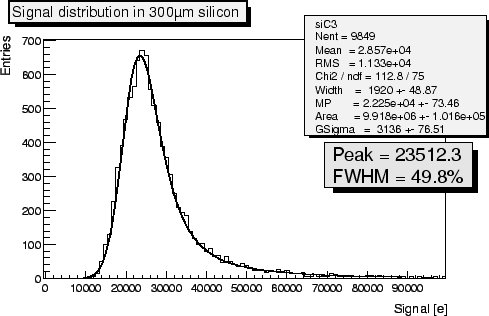
\includegraphics[width=0.6\textwidth]{\chfourteen/Landau.jpg}
 \end{center}
 \caption{Measured MIP signal distribution in a Silicon detector of 300\mum thickness.}
 \label{fig:Landau}
\end{figure}

The silicon sensor adopts a double sided n+-in-n design: pixels consist of high dose n+ implants on a high resistance n substrate.
The backside of the substrate is p-doped, therefore the p-n junction is placed on this side of the sensor. A cross-section of the sensor is shown in Fig.~\ref{fig:PixSensor}.
If the junction is reverse biased, a depletion zone forms that extends towards the pixel implants. In this zone, an electric field is established that allows ionization charge to drift. Electrons drift toward n+ implants while holes drift toward the back of the sensor. In Fig.~\ref{fig:PixSensor}, the bulk of the silicon is p-type because of the type inversion occurring in the bulk after prolonged exposure to high fluences of radiation.
In fact, the effective concentration of impurities gradually decreases with exposure, until a transition to the the other type material behavior occurs.
At this stage, the depletion zone grows from the pixel implants towards the back of the sensor, enabling the collection of electrons even when the sensor is only partially depleted.
Extremely high operating voltages can therefore be avoided, reducing the problems of leakage currents and high voltage breakdowns. Furthermore, the double-sided processing of n+-in-n detectors allows a guard ring concept which keeps all sensor edges at ground potential and avoids the risk of disruptive discharges to the very closely spaced front-end chip.

\begin{figure}[!htb]
 \begin{center}
 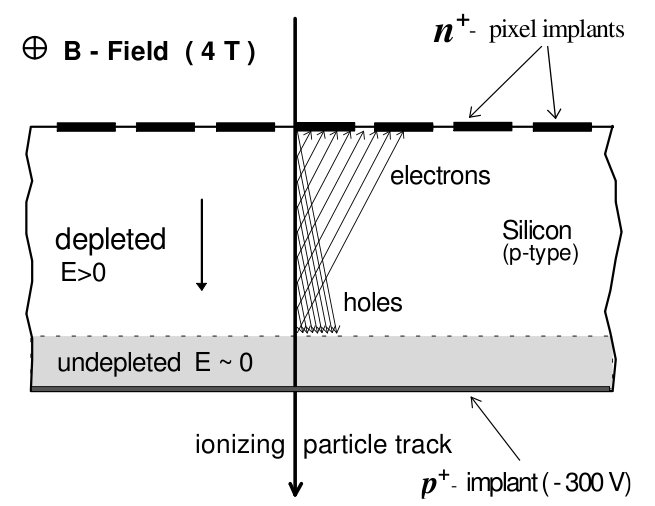
\includegraphics[width=0.5\textwidth]{\chfourteen/PixSensor.jpg}
 \end{center}
 \caption{Illustration of a charged particle crossing a sensor of the BPix detector. The charge carriers produced by the passage of the ionizing particle are collected at the high dose n+ implants.}
 \label{fig:PixSensor}
\end{figure}

Additional processing is needed on the readout side to electrically isolate the n-implants from each other.
The electron accumulation layer induced by ionizing radiation otherwise tends to short-circuit the pixel implants.
A moderated p-spray technique is used, which consists of a medium dose p-type Boron implants.\\

The position resolution of single-pixel hits is given by the pixel pitch divided by the $\sqrt{12}$
However, the spatial resolution can be improved exploiting charge sharing among adjacent pixels. A group of pixels showing a signal from the same particle is usually called ``cluster''.
Significant charge sharing is a consequence of the Lorentz drift in the strong magnetic field of 4\unit{T} inside CMS.
In fact, charge carriers released by the ionizing particle in the silicon sensor do not follow the electric field lines to the collection electrodes, but are deflected by the Lorentz force (Fig.~\ref{fig:PixSensor}).
Furthermore, the analog readout of the CMS pixel detector allows for an interpolation of the amount of collected charge for each of the pixels in the cluster.
This effects influenced the choice of the barrel pixels size in order to achieve the optimal spatial resolution.
Two-pixel clusters and interpolation allow a much better resolution, limited only by fluctuations of the charge deposition.
Since division of the signal charge among more than two pixels increases the data rate and reduces the signal charge per pixel without an improvement of the resolution, an ideal choice of the pixel size in the direction perpendicular to the magnetic field ($r\phi$) is therefore given by the length over which charges are spread when they reach the surface of the sensor.
For the usual $\sim300\mum$ sensor thickness and a Lorentz angle of $28^\circ$ this amounts to $\sim150\mum$.
A slightly smaller size of 100\mum was chosen to maintain charge sharing, and hence resolution, after irradiation.
The area of a pixel must be large enough to accommodate the readout electronics.
With one dimension fixed by the Lorentz drift, this leads to a more or less quadratic shape of $100\mum(r\phi)\time150\mum(z)$, resulting in comparable resolution in both directions.

\subsection{Readout chip}\label{subsec:BPix_ROC}

The readout chip is responsible for measuring the charge deposited by a particle in the sensor's pixel.
It amplifies and samples the signal with a time resolution of 25\unit{ns}, which is the time between two LHC bunch crossings.
The pixel hit information have to be stored on-chip during the CMS Level-1 trigger latency of 3.2\mus after which they are either readout or discarded.
Each pixel sensor is connected via a bump bond to its own readout circuit on the ROC, referred to as {\it Pixel Unit Cell} (PUC). 
The PUCs are arranged in $26\times80$ double columns. Each double column represents an independent readout unit controlled by a circuit sitting in the column periphery from where the PUC is controlled, data are buffered and global functions common to all pixels are located.
%Local bus lines connect all PUCs of a double column with the column periphery, one of them being the Column OR which combines all PUCs in the double column into a global OR.
%The PUC can be divided into an analog part and the digital logic. The signal from the sensor enters a two stage charge sensitive pre-amplifier/shaper system. The shaper is a band-pass filter that limit the bandwidth of the preamplifier output signal. This is beneficial for a reduction of high- and low- frequency noise contributions introduced in particular by the sensor leakage current and by the input device. The pre-amplifier input is DC coupled to the sensor pixels. Its feedback must absorb the expected sensor leakage current of 10 nA per pixel. This introduces a DC-offset at the preamplifier output bringing the circuit out of its operation regime. A globally programmable current source at the input node compensates for sensor leakage current.

To control and optimize the readout, 26 digital-to-analog converters (DAC) can be programmed using a serial protocol similar to I$^2$C modified to operate at 40\unit{MHz}.

The PUC can receive a signal either through a charge deposition in the sensor or by injecting a calibration signal.
Within the PUC, the signal is first passed through a two stage pre-amplifier/shaper system to a comparator where zero-suppression is performed.
It compares the shaper output to a threshold value which is programmed by a DAC distributed globally to all pixels.
Since variations of the threshold of the individual pixels caused by transistor mismatch, voltage drops or preamplifier gain variations can lead to an increased noise hit rate or to a reduced sensitivity, each pixel has a 4-bit DAC to trim the threshold. Furthermore, a mask bit allows to disable noisy pixels.
When the rising edge of the signal has passed the threshold, the signal height is sampled after some delay and stored in the sample-and-hold capacitance until the readout mechanism is started from the periphery. During this time the pixel becomes insensitive.

Since the L1 trigger latency time in CMS is 3.2\mus (128 bunch crossings), the information of a hit pixel, including the associated bunch crossing number information and the analog pixel signal, can not be kept on the pixel itself during this time without introducing a significant inefficiency. In the architecture chosen for the CMS pixel readout, referred to as {\itshape Column Drain Architecture}, the basic idea is to copy all pixel hits occurring in a pixel double column into the column periphery as soon and as fast as possible in order to free the pixels for the next hit. In this case the probability of having a second hit in the pixel during the latency is significantly reduced.
Each double column informs the column periphery immediately of any hits that occur in the double column sending to the periphery a current with adjustable intensity.
The column periphery writes the value of the bunch crossing counter into a time stamp buffer and initiates a token scan of the double column passing a readout token from cell to cell.
Once the hit pixel is found, in the readout block of the PUC the token signal initiates the transfer of pixel address and analog pulse-height information, which are stored in a data buffer located in the periphery waiting for the L1 trigger. The hit pixels remain inactive until their hit information has been transferred.
The double column periphery verifies the trigger by comparing the time stamp with a counter running behind the bunch crossing counter by the trigger delay. In case of agreement the column is set into readout mode and the data acquisition is stopped, otherwise the data are discarded. When the readout token arrives at the double column periphery the validated data are sent to the chip periphery and the double column is reset. The ROCs are read out serially via a 40\unit{MHz} analog link.

A picture of the BPix readout chip is shown in Fig.~\ref{fig:ROC}.

\begin{figure}[!htb]
 \begin{center}
 %\subfigure[]{\label{fig:ROC_a}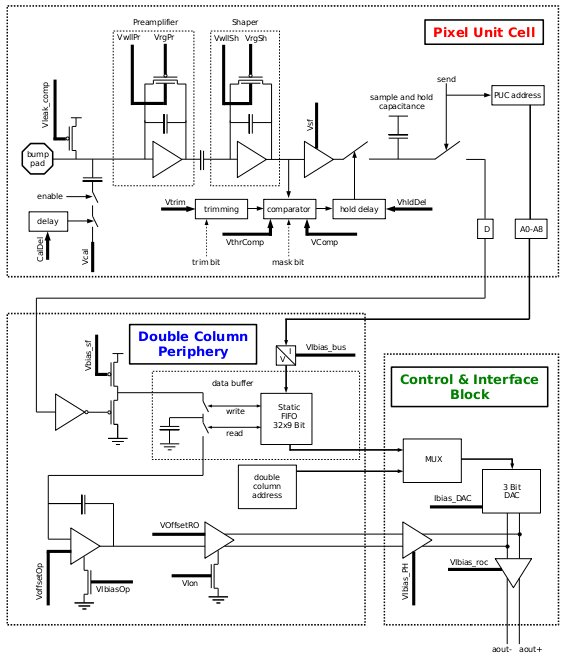
\includegraphics[width=0.37\textwidth]{\chfourteen/PUC.jpg}}
 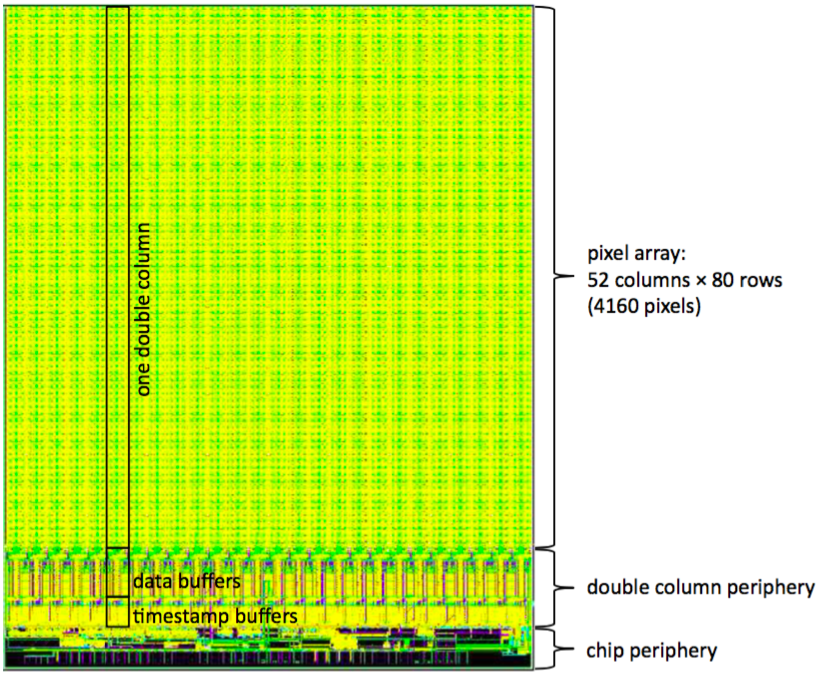
\includegraphics[width=0.6\textwidth]{\chfourteen/ROC.png}
 \end{center}
 \caption{Picture of the BPix readout chip showing the three main building blocks: double column, double column periphery and chip periphery~\cite{Chatrchyan:2008zzk}.}
 \label{fig:ROC}
\end{figure}

\subsection{Token bit manager}

A token bit manager chip is wire-bonded to the HDI and controls the readout of the ROCs.
%Since there are two analog data links per BPix module to the FED for the inner two layers, the TBM is configured as pairs in a dual TBM chip.
%The readout of several chips on a module is controlled by the Token Bit Manager (TBM) chip~\cite{Bartz:920426}.
It serves as an interface for data acquisition and programming and is responsible to synchronize the readout of the ROCs on the module.
%The main functionality of the TBM is to synchronize the data transmission.
For each incoming L1 trigger the TBM sends a token in a fixed order from chip to chip and waits until the token returns from the last chip in the chain.
The chip that has the token transmits all hits for a given trigger and then passes the token to the next chip.
Each ROC starts sending a three clock cycle header when it receives the readout token.
While the header is transmitted, the token is passed through the chip looking for a double column with validated hits belonging to that token.
The length of the header is sufficient for the token to skip all 26 double columns if no triggered hits were present and to be passed on to the next chip with the right timing.
Triggers and readout tokens are both counted and hits are only readout when the token number matches the readout number.
It must be ensured that exactly one token for every trigger is issued and that there is never more than one token.
The ROCs in the module are either serviced by a single token that sequentially passes through all the 16 chips, or a second channel in a dual TBM chip is used such that the ROCs are divided into two groups of eight.
This method is employed for the two innermost layers of the detector which experiences higher hit rates per module than the others.
This requires two separate buses for the ROC readout, and the data streams are also individually transmitted through two separate readout links for the data acquisition. 
The two modes of operation are illustrated in Fig.~\ref{fig:TBMreadout}.
The TBM keeps track of triggers arriving while the token is still under way with a trigger stack of 32 entries that is filled each time a trigger arrives and reduced every time a token returns.
In case of a stack overflow, the TBM withholds the incoming triggers from the ROCs until the stack is reduced. It notifies the data acquisition that events have become lost in this case.
The TBM multiplexes the signal from the ROCs, adds a header and a trailer to the data stream and drives the signal through the readout link. In addition, the TBM distributes the L1 trigger and the clock to the ROCs.
The header contains an event number and the trailer a status information, such as the stack stack overflow warning.
%A loss of a token destroys the synchronization between module and data-acquisition, effectively leading to the loss of all subsequent data. The trigger counter is used to verify the correct synchronization.
%A schematic of the readout chain is displayed in Fig.~\ref{fig:TBMreadout}.
The TBM chip also includes a communication component called the HUB which serves as a port for programming commands sent from the DAQ.

\begin{figure}[!htb]
 \begin{center}
 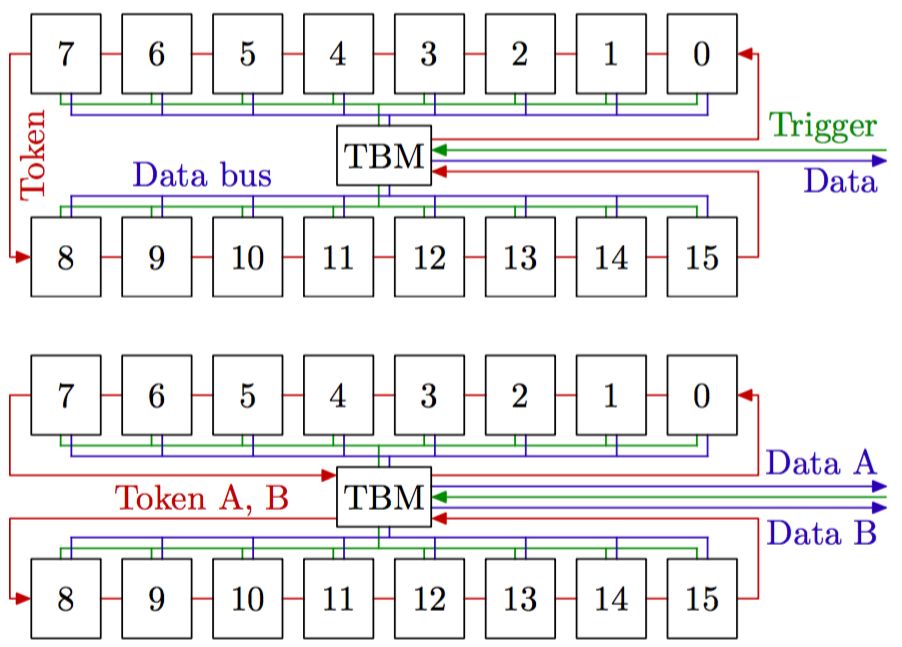
\includegraphics[width=0.6\textwidth]{\chfourteen/TBMreadout.png}
 \end{center}
 \caption{Illustration of the mechanism for the readout of the ROCs on a module. The readout is initiated by the TBM after the occurrence of a trigger. In the upper scheme, a token is sent to a group of 16 ROCs.
 In the lower scheme, two separate tokens are each sent to a group of 8 ROCs. In this case, two data links are required for data transmission.}
 %\caption{Schematics of a readout chain consisting of a TBM and a group of ROCs~\cite{Bartz:920426}.}
 \label{fig:TBMreadout}
\end{figure}

%%%%%%%%%%%%%%%%%%%%%%%%%%%%%%
\section{Detector readout and control}\label{sec:BPix_DAQ}
%%%%%%%%%%%%%%%%%%%%%%%%%%%%%%

%A schematic drawing of the pixel readout and control systems is shown in Fig.~\ref{fig:BPixSystem} and a detailed description can be found in Ref.~\cite{Kotlinski200673}.
The two most important front-end components placed on detector modules are the ROCs and the TBMs introduced in the previous section. 
The signal cables from the modules are plugged into the end-flange that exists on both sides of the barrel and connects the three layers to the detector supply tubes. 
A supply tube is divided into 8 sectors which contain the power lines and the readout and control electronics of two readout groups, one serving the modules of the first two layers, the other serving the modules of the third layer.

A schematic drawing of the pixel readout and control systems is shown in Fig.~\ref{fig:BPixSystem}.
The path on the right shows the readout part of the system.
Signals from a group of ROCs are amplified and converted into a 40\unit{MHz} analog optical signal in the analog opto-hybrid circuits mounted on the supply tube.
Optical fibres allow the data to be transferred over approximately 60\unit{m} distance to the underground counting room, where a VME front-end driver unit (FED) digitize the signal, build event fragments and send them to the DAQ.
The signal path in the middle shows the fast detector control link.
In the counting room, the control signals are driven by front-end control (FEC) units which are used to program the detector modules.
The signals enter the supply tubes through optical fibres to be converted in digital opto-hybrid circuits.
Several other electronic devices are needed by the system and are placed on the supply tubes.
Some of these components need to be programmed. This happens through a dedicated slow control link corresponding to the signal path on the left.
Also shown in Fig.~\ref{fig:BPixSystem} is the Timing Trigger and Control (TTC)~\cite{Taylor:592719} system which distributes the clock and trigger signals to all detector components.
The individual electronic devices of the pixel readout and control system are described in more detail in the following.

\begin{figure}[!htb]
 \begin{center}
 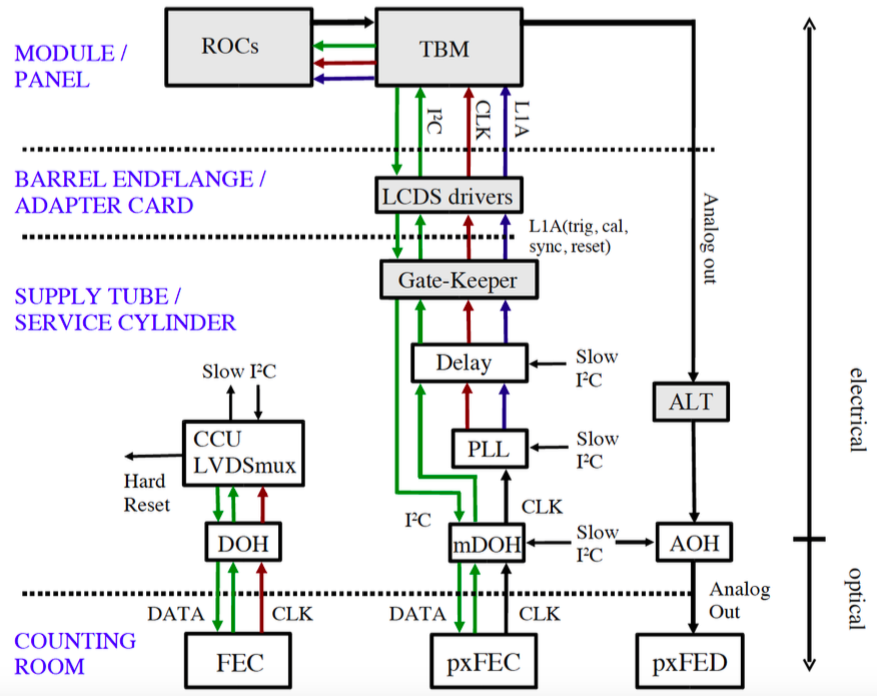
\includegraphics[width=0.7\textwidth]{\chfourteen/ReadoutAndControl.png}
 \end{center}
 \caption{Overview of the BPix readout and control system.}
 \label{fig:BPixSystem}
\end{figure}

%\subsection{Analog readout}
\subsection{Readout of the analog signal}\label{subsec:BPixReadout}

An example of an analog readout signal of a module with a single pixel hit is shown in Fig.~\ref{fig:ModuleReadout}.
The TBM header uses eight clock cycles and starts with three ultra black levels (UBL). An UBL is simply a large negative signal level well outside of the range of pixel data.
The three UBLs are followed by a black level, which defines the zero level of the differential analog signal.
The four remaining clock cycles encode an 8-bit event number.
The minimal readout of each ROC starts with an UBL, a black level and a level called last DAC which represents the value of the most recently programmed DAC.
%This sequence unambiguously identifies the beginning of a new chip in a sequence of analog levels. No further chip ID is present in the data stream. The chip number is simply incremented for each ultra black signal recorded.
A pixel hit adds a block of six clock cycles to the ROC minimal readout: two for the double-column address, three for the row address, and one for the pulse-height.
In order to speed up the transmission of digital pixel hit information while maintaining the global 40\unit{MHz} clock,
the pixel addresses are not sent in a common binary fashion, but the available signal amplitude is divided into six possible analog levels ( (2.5 bits/clock)).
%The pixel addresses are not binary coded, but use a set of six discrete analog levels (2.5 bits/clock).
The readout is terminated by the TBM trailer, containing two UBLs, two black levels, and four clock cycles with the TBM status information.
The data stream which contains all hit information belonging to a single trigger is sent out by the TBM through the module Kapton cable.
%The Kapton cable consists of differential analog lines separated by quiet lines from the lines for the fast digital signals.
%The analog signals are split from the digital signals on the endring PCB.
%The TBM sends the data over kapton and PCB traces to the Analog Optohybrids [5], where levels are amplified and shifted and then converted to a laser drive current with adjustable gain and threshold.
Kapton cables bring the analog signals to the printed circuit board (PCB) on which the analog optical hybrids (AOHs)~\cite{1221923} are placed.
The electric analog signals are amplified in an Analog Level Translator (ALT) chip and converted into 40\unit{MHz} analog optical signals in the AOHs.
Each AOH is equipped with 6 lasers with adjustable gain and threshold, which drive the signal through optical fibers to the front end drivers.

\begin{figure}[!htb]
 \begin{center}
 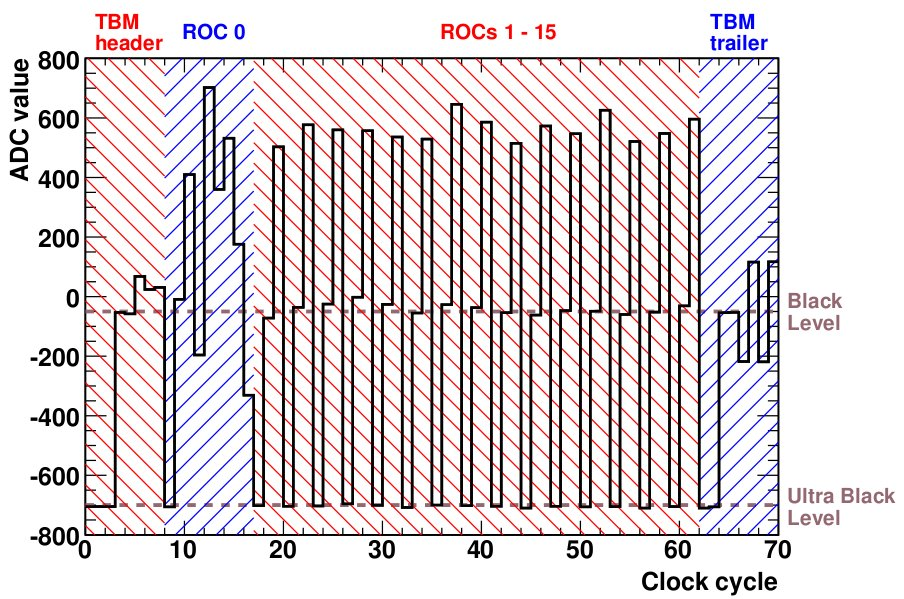
\includegraphics[width=0.6\textwidth]{\chfourteen/analogueRO.jpg}
 \end{center}
 \caption{Analogue readout of a pixel module with one hit in ROC 0.}
 \label{fig:ModuleReadout}
\end{figure}

%\subsection{Front end driver}
A total of 32 FED modules~\cite{Pernicka:1091743}, located in the underground counting room, receive the data packets.
They convert the signals from optical to electrical, perform the digitization at the LHC frequency, and decode the pixel hit information.
The pixel FED also builds event fragments and sends them to the CMS central DAQ system.
It is a 9 U VME module that includes optical receivers, ADCs and several FPGAs for signal processing.
It has been designed at HEPHY Vienna.

A FED has three opto-receiver devices each of which has twelve input channels where the fibers terminate. Each input channel is equipped with a 10-bit ADC.
The ADC has a clock with adjustable phase w.r.t. the global clock in steps of 1.6\unit{ns} to select the optimum digitization sampling point for each input.
A programmable offset voltage can be set for each optical input in order to compensate for bias shifts in the analog signal.
%such that the digitization point can be optimized for each channel which is essential to maintain a good signal-to-noise ratio. 
An additional, single optical input receives TTC signals such as clock, trigger and reset.
Each channel has a 1k words 32-bit data buffer (FIFO1) which stores the ``raw'' module signal (Fig.~\ref{fig:ModuleReadout}).
The data package from four or five (depending on the location) FIFO1 channels are transferred in a FIFO2 with a size of 8k words and a width of 64 bits plus 4 control bits.
During the data transfer to FIFO2 the input event number is compared with that of the CMS TTC system.
The data of all FIFO2 memories are collected by two final memories (FIFO3) of 8k words each over two buses of 64+4 bits at 40\unit{MHz}. 
Four front FPGAs, each handling 9 inputs, house FIFO1 and FIFO2 buffers, while a center FPGA houses the final FIFO3 where the event fragment is collected,
together with the S-link connection to the central DAQ.
The FED can also be operated in a transparent mode making unprocessed ADC output data available for calibration and testing purpose. 

\subsection{Detector control and programming}

The detector control and programming is performed through front-end control modules (pixel FECs or pxFEC) located in the underground counting room.
The function of the pixel control system is to send the 40\unit{MHz} clock, the trigger and control signals (e.g. resets) to the front-end electronics,
and to program all front-end devices (TBMs and ROCs).
All the signals are sent through optical fibers and converted to electrical signals by digital optical hybrids (DOHs)~\cite{1221923} mounted on the supply tube before forwarding them to the pixel modules.
%Each FEC is housed in a 9 U VME card.
%The FEC card has been designed by the CERN microelectronics group.
%The FEC card consists of a mother card with 8 daughter cards, called mFECs. Each mFEC contains an optical transceiver and an FPGA for the protocol.
%%%
%Each DOH contains two laser drivers and two PIN diodes. The DOH is mounted on a PCB together with other devices needed in the system.
%In particular, a phase locked loop (PLL) chip is used to split the clock from the trigger, and the DELAY25 chips adjust the relative phases of all control signals.
%The Gate-Keeper chip converts the LVDS signals used by PLLs and DELAY25s to low current differential signals (LCDS) used by the pixel front-end chips.
%%%
%Finally, the LCDS-driver chips mounted on the endring PCB are used to drive the signals on the Kapton cables to each detector module. In addition, these chips are used to compensate the signal phases for the different Kapton cable lengths.
%The two front-end chips, ROCs and TBMs, need a large number of parameters to be downloaded. The TBM chip has 11 8-bit DACs and registers. With the total number of 1000 TBMs about 10kBytes of data will have to be downloaded. One ROC chip has 28 8-bit DACs and registers, giving for the total number of 15 k ROCs about 450 kBytes. However, the required download data volume is completely dominated by the pixel thresholds. Each pixel has a programmable threshold called trim. With 66M pixels about 66MBytes have to be downloaded to the front-end.
A DOH is connected to four optical fibers, two for receiving and two for sending signals. The LHC 40\unit{MHz} clock and trigger information is encoded in one signal which is sent over a single fiber to the DOH. 
A modified version of the common I$^2$C protocol has been developed to cope with the required volume of the data that have to be downloaded to configure the front-end.
The main modifications include the increase of the clock speed to 40\unit{MHz} and dropping the requirement of an acknowledge signal.
Each DOH contains two laser drivers and two PIN diodes. The DOH is mounted on the digital opto-board together with other electronic devices needed in the system.
In particular, a phase locked loop (PLL) chip~\cite{PLLmanual} is used to split the clock from the trigger, and the Delay25 chips~\cite{Delay25manual} adjust the relative phases of all control signals.
The Gate-Keeper chip converts the LVDS signals used by PLLs and Delay25s to low current differential signals (LCDS) used by the pixel front-end chips.
Finally, the LCDS-driver chips mounted on the end flange PCB are used to drive the signals on the Kapton cables to each detector module.
In addition, these chips are used to compensate the signal phases for the different Kapton cable lengths.\\

The electronics on the supply tubes (DOHs, PLLs, Delay25s, AOHs, and so on) have to be controlled and programmed.
%In addition to the pixel specific devices several other components like PLLs, AOHs, and others, have to be controlled and programmed.
This is achieved through a system of four CCU (Communication and Control Unit) boards equipped with 9 CCU chips~\cite{Paillard:593914}.
This is indicated in Fig.~\ref{fig:BPixSystem} as ``slow I$^2$C'', since the standard I$^2$C protocol is implemented for this task.
The boards are mounted on the supply tubes and each of them supervises one quarter of the detector.

The slow control links are implemented as a ring architecture.
A ring consists of 9 CCUs, two optical drivers and receivers that bring clock, trigger and control data to the CCUs
and a front-end controller (tracker FEC or tkFEC)~\cite{Gill:921198}
providing the communication with the CCUs and the programming signals.

Each CCU distributes the digital control signals to a set of individual boards forming one read out sector of the detector.
A CCU chip supports two I$^2$C channels to communicate with the front-end electronics, and three PIA channels to generate the necessary signals to reset the circuits and the ROCs of one sector..
Eight CCUs are used for the control of the eight sectors, the ninth CCU is a dummy chip used for redundancy.
Since a large number of front-end channels depend on the same control link, a very high reliability of the system is of utmost importance.
A CCU failure leads to a loss of communication to all electronics attached to it.
A redundancy scheme based on doubling signal paths and bypassing of interconnection lines, between the CCUs and between the CCUs and the FEC, is supported.
The dummy CCU allows to mitigate a single DOH failure. The CCU is equipped with two DOHs which form separated control rings and thus ensure a high operational reliability.
The DOHs on the CCU board are programmed by the first two CCU chips.

\subsection{Supply tubes}
%\subsection{Communication and control unit}

As mentioned previously in this section, the readout and control circuits of the pixel detector are integrated on four supply tube half cylinders.
In addition the supply tubes bring the power and cooling lines to the detector.
A schematic view of a supply tube half cylinder is shown in Fig.~\ref{fig:SupplyTubes}.
%Starting from the detector side, each sector of the supply tube includes an analog opto-board with six AOHs and a digital opto-board with two DOHs.
One sector includes an analog opto-board with six AOHs, a digital opto-board with two DOHs, two PLL chips, two Delay25 chips and two Gate-Keeper chips.
A total of 192 AOHs and 72 DOHs are used for the pixel barrel detector. For each sector, 44 optical fibers drive the communication with the front-end modules, 36 for the analog readout and 8 for the digital control. 
%The barrel pixel readout system is organized into 64 independent readout groups consisting of analog and digital opto-hybrid circuits which serve 8, 12 or 16 modules.
The CCU board is placed in the central sector of the supply tube.
  
 The stability of the analog signal is strongly affected by the temperature dependence of the AOHs.
A shift of 50 ADC counts is observed in the level of the analog signal for a temperature variation of the AOH of $1^\circ$\unit{C}.
The FED is able to internally correct for a drift within a temperature range of $\pm2^\circ$\unit{C}.
Consequently, the temperature of the AOHs has to be controlled within a very narrow range in order to assure a stable operation of the detector.
The barrel pixel supply tubes are equipped with a total of 124 temperature sensors and 8 humidity sensors.
The temperature sensors are placed on the CCU boards, the AOH motherboards and on the supply tube cooling lines.

\begin{figure}[!htb]
 \begin{center}
 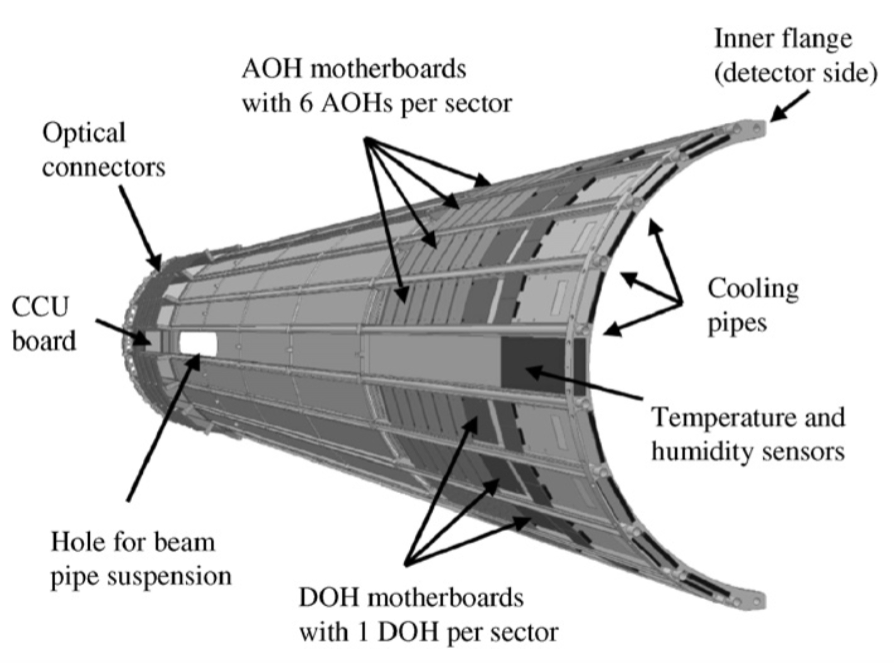
\includegraphics[width=0.6\textwidth]{\chfourteen/SupplyTubes.png}
 \end{center}
 \caption{Drawing of a supply tube half-cylinder~\cite{Kastli2007724}.}
 \label{fig:SupplyTubes}
\end{figure}

%%%%%%%%%%%%%%%%%%%%%%%%%%%%%%
\section{Pixel Online Software}\label{sec:BPix_POS}
%%%%%%%%%%%%%%%%%%%%%%%%%%%%%%

\begin{figure}[!htb]
 \begin{center}
 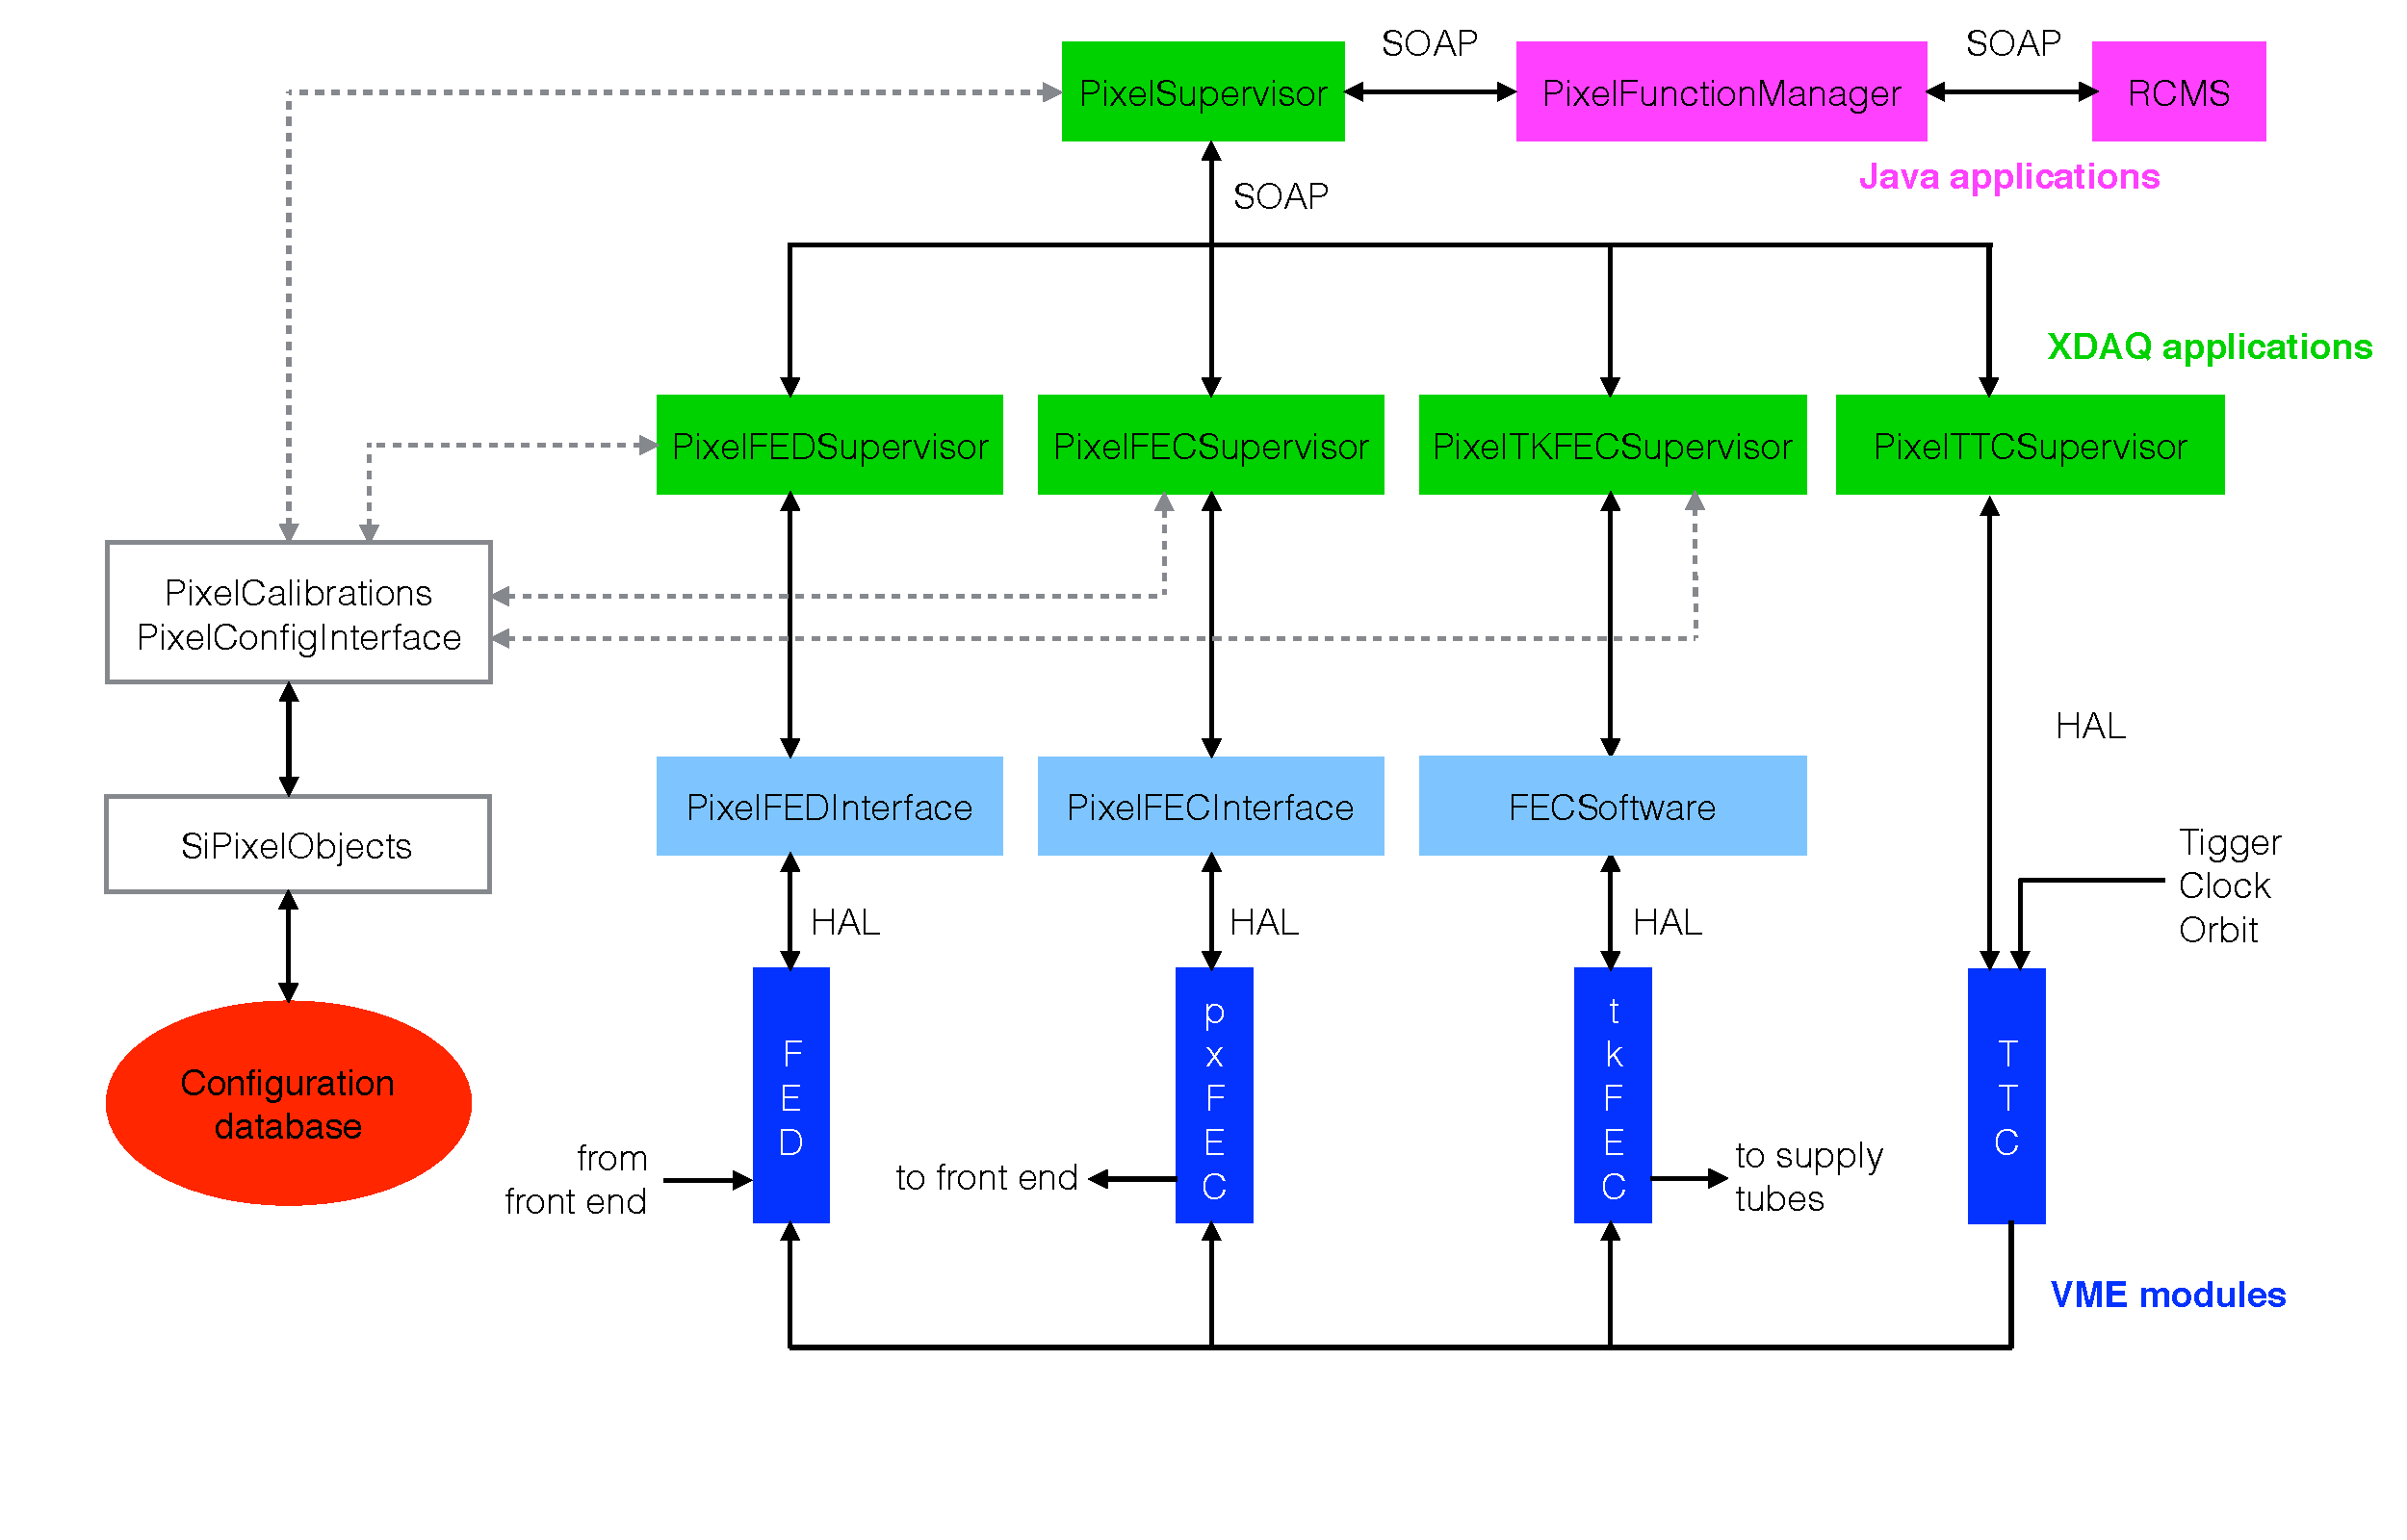
\includegraphics[width=0.7\textwidth]{\chfourteen/POSscheme.pdf}
 \end{center}
 \caption{Illustration of the dependencies among the main applications and packages implemented in the pixel online software.}
 \label{fig:POS}
\end{figure}

This section describes the design and implementation of the pixel online software, used for controlling and calibrating the CMS pixel detector.
Its main functionalities are to configure the detector, perform calibrations, analyze calibration data and monitor the detector during data taking.
The pixel online software is based on the XDAQ toolkit~\cite{Brigljevic:2003kg} and is written in C++. It has a very complex structure built from a large number of different applications and packages.
The dependencies among the main applications and packages is presented in Fig.~\ref{fig:POS}.
%The supervisor applications are at the top and depend on the packages below.
The top level application is represented by the \texttt{PixelSupervisor} which is responsible for the overall coordination of the pixel DAQ.
%The PixelSupervisor talks to the supervisors that directly control the hardware.
Its main function is to coordinate the activities of the other supervisors, particularly during configuration and calibration.
It is also responsible for updating the configuration database with new settings obtained by calibrations.
Among the other supervisors there is the \texttt{PixelFECSupervisor} that controls the pxFECs and is responsible for loading the configuration parameters for the ROCs and TBMs from the configuration database and programming those parameters into the detector.
Similarly, the \texttt{PixelTKFECSupervisor} controls the tkFECs and the initialization of all the electronics placed on the supply tubes. The \texttt{PixelFEDSupervisor} controls the FEDs.
%The other supervisors are the PixelFECSupervisor and the PixelTKFECSupervisor that control the pixel and tracker FECs, respectively, as well as the PixelFEDSupervisor controlling the FEDs. 
A set of classes such as \texttt{PixelFEDInterface}, \texttt{PixelFECInterface}, and so on, provides the direct communication between the supervisors and the VME hardware via Hardware Access Library (HAL)~\cite{HAL}.
An additional supervisor is included in the software that controls the pixel TTC module used for trigger and timing. Among other things the TTC module is used during calibrations to generate triggers.
The various supervisors run as independent processes, or even on different computers. Therefore, in order to communicate with each other they must exchange messages on the network. This is done using the XML-based SOAP (Simple Object Access Protocol) protocol.
A function manager acts as an interface between the global run control (RCMS, Run Control and Monitoring System) and POS.
It is a JAVA application that basically passes the state machine of CMS (Halted, Running, Configured, and so on) to the \texttt{PixelSupervisor} which then forwards state requests to the underlying supervisors to carry out the different tasks needed in state transitions of the run control.
Another key element of the software is represented by the \texttt{PixelConfigInterface} package which provides access methods for retrieving and storing configuration data.
Several different classes are available in the \texttt{SiPixelObjects} package, each responsible for storing a specific set of detector settings as well as the configuration needed by the calibration code (ex: which detector parameter to scan and its range).
For instance, the \texttt{PixelNameTranslation} class translates from the naming scheme used to label each individual ROC to the hardware addresses used by both the FEC and the FED to identify a specific ROC.
Similarly, the \texttt{PixelDACSettings} and \texttt{PixelTBMSettings} classes store, respectively, the DAC settings for all ROCs on one module and the settings for one TBM.
The \texttt{PixelSupervisor} features a web GUI that can be accessed as an html page.
It displays information about the current configuration, or if it is not configured it allows the user to select a possible configuration from a list and configure the detector using that choice.
The picture in Fig.~\ref{fig:PixGUI} shows an example of the GUI illustrating the list of configurations, each corresponding to a detector calibration.
The calibration routines are implemented in independent and separate classes contained in the \texttt{PixelCalibrations} package.
The description of the detector calibration procedures is presented in the following chapter.

\begin{figure}[!htb]
 \begin{center}
 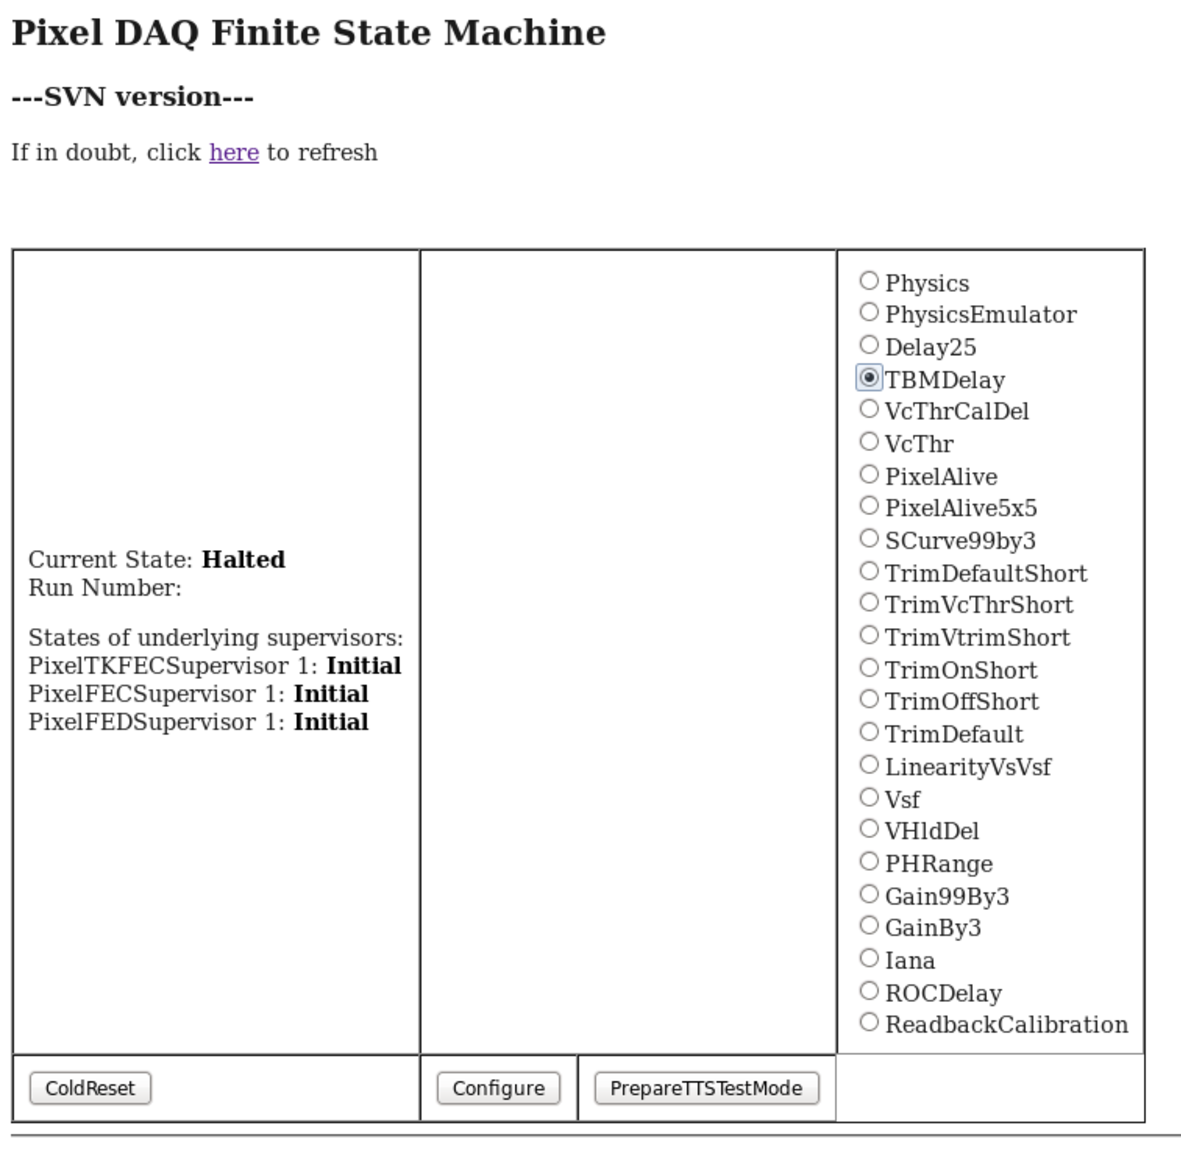
\includegraphics[width=\textwidth]{\chfourteen/PixelSupervisor.pdf}
 \end{center}
 \caption{Example of the \texttt{PixelSupervisor} GUI showing the list of configurations each corresponding to a detector calibration.}
 \label{fig:PixGUI}
\end{figure}

%\section{Performance at $\sqrt{s}$ = 8 and 13 TeV}